\section{Semaine 10 : 10/04/2023 - 14/04/2023}
\graphicspath{{semaines/semaine_10/images/}}

\begin{abstract}
	(Lundi est férié)
	
	Après discussion avec Michel et Emmanuel mardi matin, on a discuté de quelques points qu'il faudrait traité suite aux résultats obtenus avec PhiFEM :
	\begin{enumerate}[label=\textbullet]
		\item On garde la fonction $\phi_c(x,y)=||x-0.5||_\infty-0.5$ pour construire les ensembles utilisés par PhiFEM. On utilise la levelset suivante pour PhiFEM : $\phi(x,y)=x(1-x)y(1-y)$.
		\item On effectue les courbes de convergence de PhiFEM sur le carré et sur le cercle pour ce problème. On étudiera également les erreurs d'interpolation.
		\item On cherchera ensuite à comparer les résultats FEM et PhiFEM. En effet, la semaine dernière on a considéré le même problème pour les deux méthodes mais les résultats obtenus sont très différents.
		\item Pour finir, Michel a proposé une analyse pour la sortie du FNO : la décomposition en série de Fourier de la solution (ce qui nous permettrait de déterminer dans lequel des cas on se trouve, parmis ceux observés sur la solution analytique et ainsi d'avoir une idée de la forme de la perturbation en sortie du FNO). Problème : Je ne comprends pas ce qui nous garantit que l'on peut faire cette décomposition, la sortie n'est pas forcément périodique !
	\end{enumerate}
	On a également remarqué qu'il faut penser à prendre un epsilon de tolérance pour la construction des espaces (car si la la levelset se situe exactement à l'intersection de deux cellules il peut y avoir des problèmes d'arrondis).
\end{abstract}

Dans la suite, on construira les ensembles $\mathcal{T}_h^\Gamma$ et $\mathcal{F}_h^\Gamma$ en utilisant la fonction :
$$\phi_c(x,y)=||x-0.5||_\infty-0.5$$
Cependant, dans la résolution PhiFEM, on considérera :
$$\phi(x,y)=x(1-x)y(1-y)$$

\subsection{Convergence PhiFEM}

On obtient les résultats suivant pour deux cas de fréquence (à gauche sur le carré, à droite sur le cercle) :

\begin{minipage}{\linewidth}
	\centering
	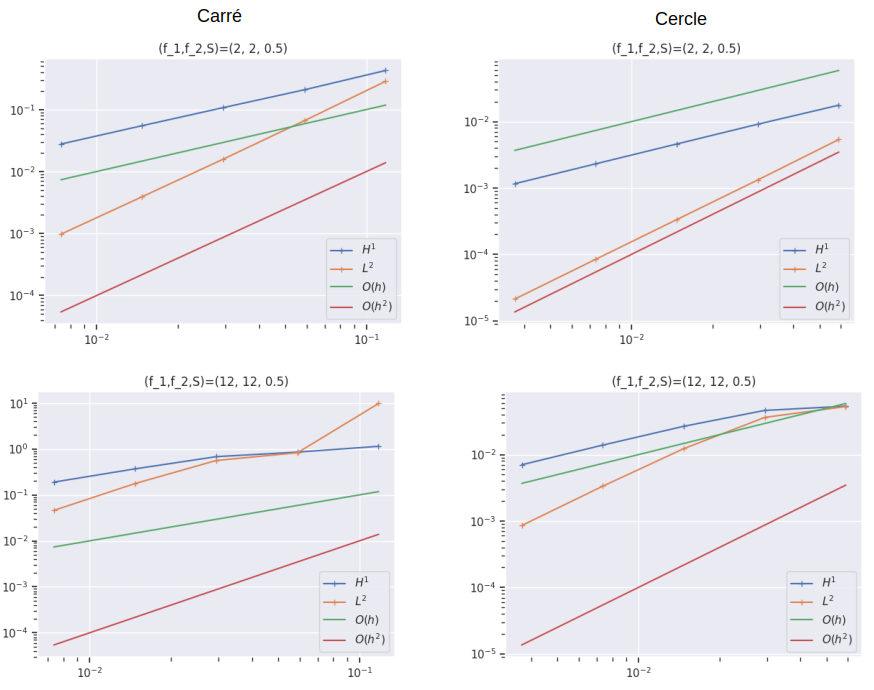
\includegraphics[width=0.7\linewidth]{convergence.png}
\end{minipage}

\subsection{Comparaison FEM-PhiFEM}

Les résultats de la semaine dernière était plutôt étranges. C'est pour cela qu'on a raisonnée en deux parties : On commence par essayer de comprendre pourquoi la correction (sans rehaussement $m=0$) fournit d'aussi bon résultat. Puis on s'intéressera au rehaussement.

\subsubsection*{Correction avec PhiFEM}

Il semblerait que lorsque l'on prend $f=f_p$, PhiFEM fournit les mêmes résultats que si on lui fournissait la solution exacte comme levelset. Si $f=f_p$ alors $P=u_ex$ et donc 
$$u_p=u_{ex}+\epsilon P=(1+\epsilon)u_{ex}$$

Il semblerait que faire varier $\epsilon$ n'ait alors pas d'effet sur l'erreur $L^2$ PhiFEM contraiement à FEM standard.

Cependant, en prenant des fréquences différents pour la solution analytique et la perturbation, on obtient les résultats attendus, à savoir que plus $\epsilon$ est petit et meilleure est l'erreur. 

Voici les résultats obtenus pour différents $\epsilon$ :

\begin{minipage}{\linewidth}
	\centering
	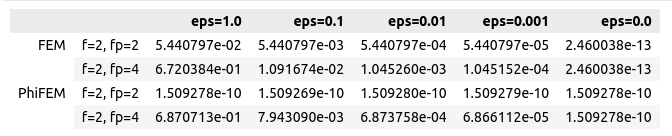
\includegraphics[width=0.8\linewidth]{comp_FEM_PhiFEM.png}
\end{minipage}

\subsubsection*{Rehaussement}

On cherche ici à comparer les erreurs FEM et PhiFEM lorsque l'on rehausse le problème. On testera pour différentes fréquences (avec $f\ne f_p$), différents rehaussement $m$ ainsi que différents $\epsilon$.

Voici les résultats numériques obtenus :

\begin{minipage}{\linewidth}
	\centering
	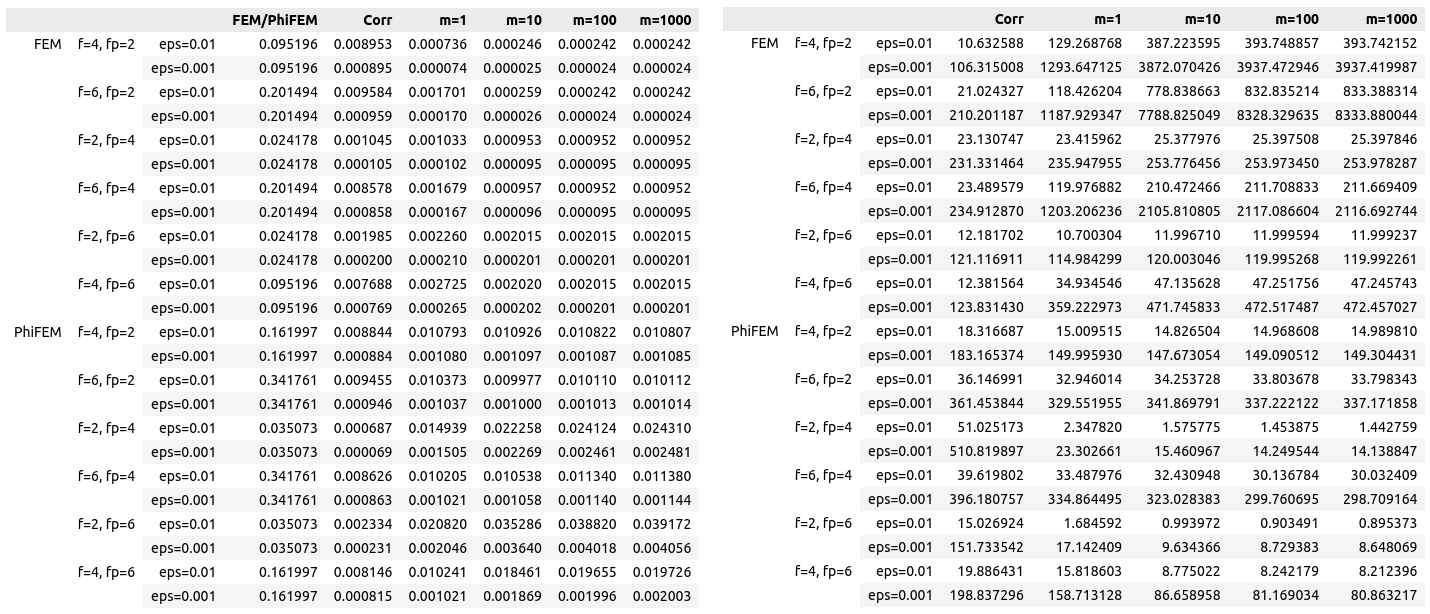
\includegraphics[width=\linewidth]{comp_FEM_PhiFEM_2.png}
\end{minipage} \\

Voici les résultats obtenus avec FEM à gauche et PhiFEM à droite :

\begin{minipage}{0.48\linewidth}
	\centering
	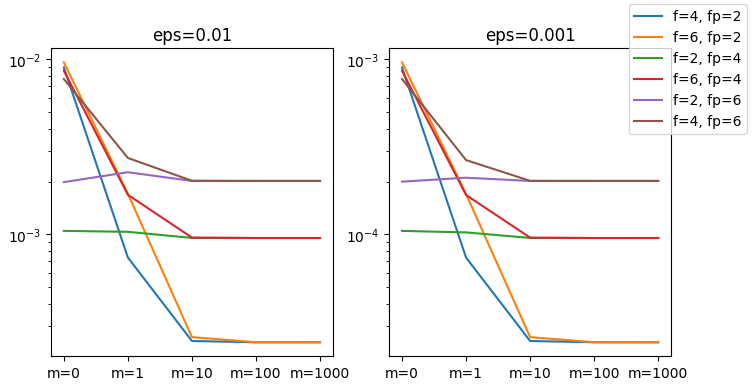
\includegraphics[width=\linewidth]{erreur_FEM.png}
\end{minipage}
\begin{minipage}{0.48\linewidth}
	\centering
	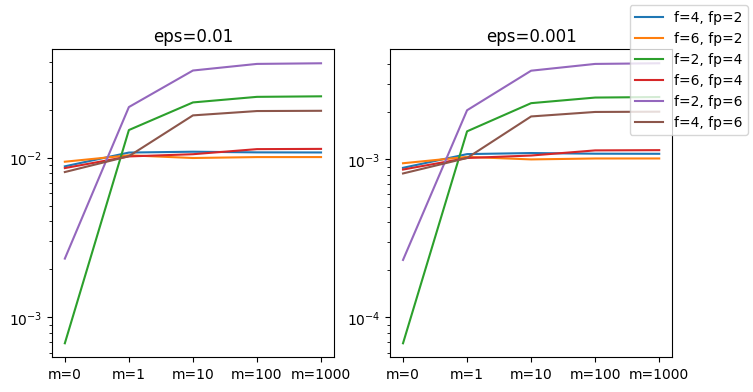
\includegraphics[width=\linewidth]{erreur_PhiFEM.png}
\end{minipage}

\subsubsection*{Variation des termes dans la formulation variationnelle}

On cherche ici à comparer les erreurs PhiFEM avec tous les termes dans la formulation variationnelle, sans les termes de stabilisation et sans  le terme de bord lorsque l'on rehausse le problème. On testera pour différentes fréquences (avec $f\ne f_p$), différents rehaussement $m$ et on prendre $\epsilon=1e-2$.

Voici les résultats numériques obtenus :

\begin{minipage}{\linewidth}
	\centering
	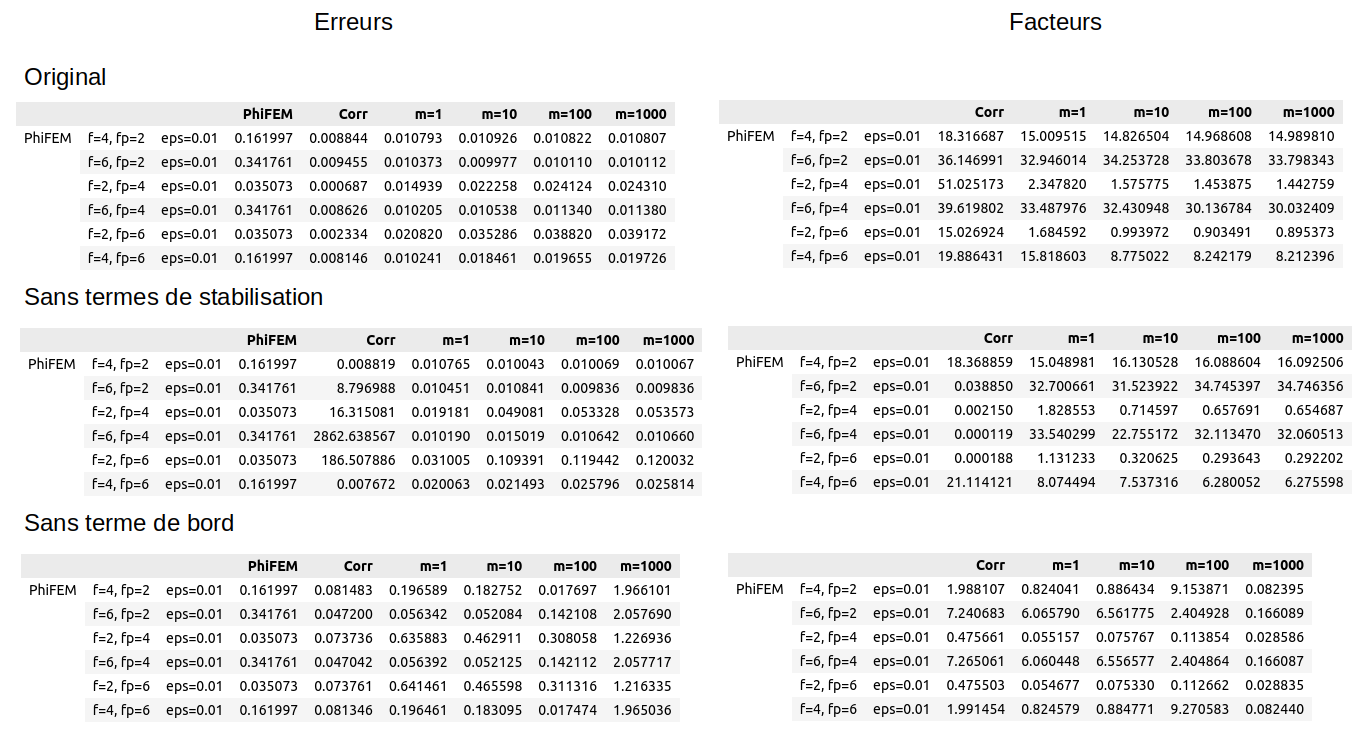
\includegraphics[width=0.9\linewidth]{tests_termes.png}
\end{minipage} \\

Voici les résultats obtenus pour les erreurs :

\begin{minipage}{\linewidth}
	\centering
	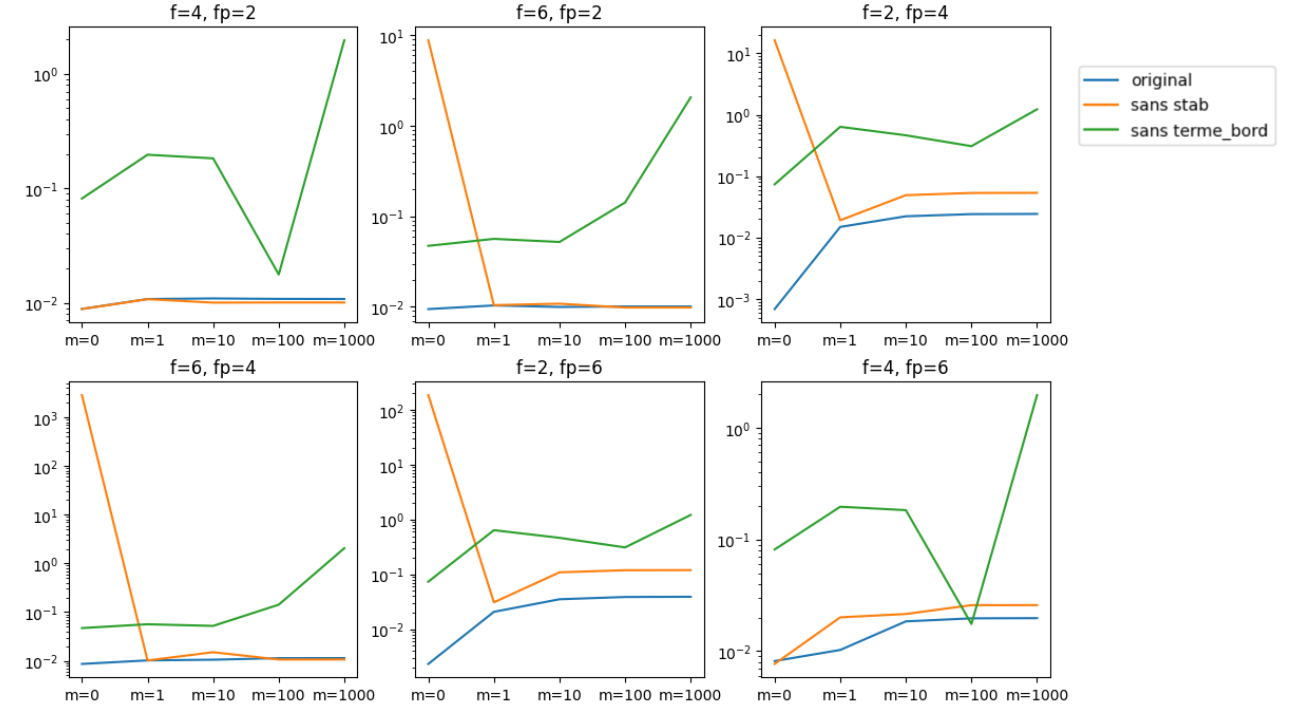
\includegraphics[width=0.72\linewidth]{tests_termes_erreurs.png}
\end{minipage}

Voici les résultats obtenus pour les facteurs :

\begin{minipage}{\linewidth}
	\centering
	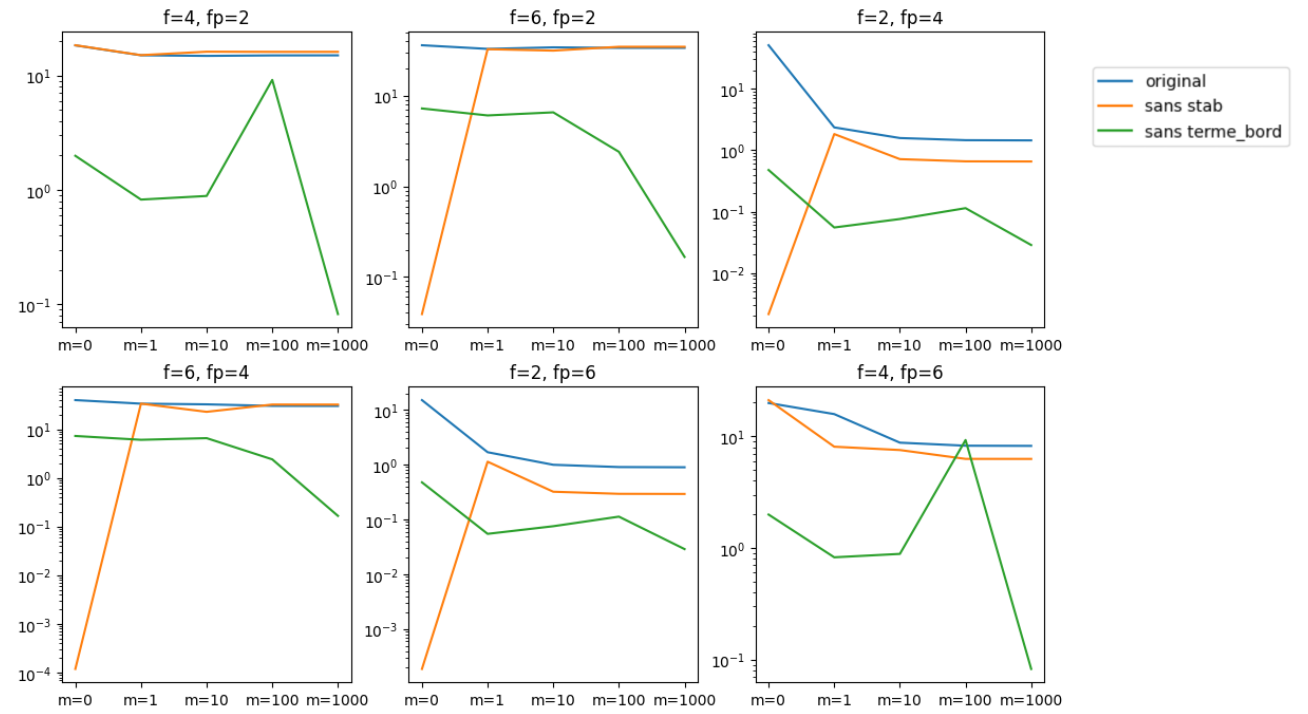
\includegraphics[width=0.72\linewidth]{tests_termes_facteurs.png}
\end{minipage}